\graphicspath{{imgs/}}

%===============================================================================
\chapter{Introduction}
%===============================================================================



In \cite{Batchelor} we believe.


%-------------------------------------------------------------------------------

\section{Flow-assist droplet assembly}

material science,
photonic crystals,
microfluidics,
lab-on-a-chip.


\section{Liquid-infused surfaces}

drag reduction,
surface engineering,
superhydrophobicity,
lubricant-infused surfaces.


\section{Suspension flows}

particle suspensions,
complex fluids,
rheology,
shear thickening.

\thesisstructure Add here a brief description of the structure of the thesis.



%===============================================================================
\chapter{Microhydrodynamics}
%===============================================================================


This chapter summarizes the mathematical formulation and theoretical basis of microhydrodynamics and particle interactions.
By \emph{particle}, we loosely mean a solid or liquid body of micron to millimetre in size, which may also be referred to as \emph{droplet} for abuse of language.
As preliminaries, most of the contents below are given without any proof. The interested reader is encouraged to read \cite{Batchelor, hb, ps, kim_karrila, graham_2018} for greater details.

\bigskip

To begin with, recall the incompressible \emph{Navier-Stokes equations}
\begin{subequations} \label{eq:Navier-Sotkes}
 \begin{equation}
   \nabla \cdot {\bm u} = 0,
  \label{eq:div-free}
 \end{equation}
 \begin{equation}
   \rho \bigg(\frac{\partial {\bm u}}{\partial t} + {\bm u} \cdot \nabla {\bm u} \bigg) = -\nabla p + \mu \nabla ^2  {\bm u} + {\bm f},
  \label{eq:NS}
 \end{equation}
\end{subequations}
relating the flow velocity $\bm u$ with the pressure $p$ in the presence of some force density $\bm f$, where $\rho$ and $\mu$ are the density and dynamic viscosity of the fluid, respectively.
Eqs.\ \eqref{eq:Navier-Sotkes}, together with appropriate boundary conditions, govern the dynamics of a Newtonian fluid that satisfies\footnote{The present thesis only concerns the Newtonian fluid as the solvent, though a particle suspension may exhbit non-Newtonian behaviours as we will see.}
\begin{equation}
 \begin{aligned}
   {\bm \sigma} = -p {\bm I}+ \mu \bigg( \nabla {\bm u} + (\nabla {\bm u})^T \bigg),
 \end{aligned}
\end{equation}
where $\bm \sigma$ is the stress tensor, and $\bm I$ the identity matrix.

Depending on the bounding material, conditions on the velocity or stress may be prescribed as boundary conditions. In the case of a solid wall, it is usually the \emph{no-slip} velocity condition; while in the case of a liquid interface, the following stress condition shall be satisfied,
\begin{equation} \label{eq:stress-bc}
  {\bm n} \cdot ({\bm \sigma}_+ - {\bm \sigma}_- )  = \gamma \kappa {\bm n} - \nabla \gamma,
\end{equation}
where $\bm n$ denotes the unit normal vector across the liquid interface (from the $-$ side to the $+$ side), $\gamma$ the surface tension coefficient, and $\kappa$ the curvature of the interface (\eg $\kappa=2/a$ for a sphere of radius $a$). 

Eq.\ \eqref{eq:NS} can be further non-dimensionalized, using the reference length $L$, velocity $U$, time $T$, pressure $P \equiv \mu U/L$, and force density $F \equiv P/L$ scales, into
\begin{equation}
   \textrm{Re} \bigg(\textrm{Sr}^{-1} \frac{\partial \hat{\bm u}}{\partial \hat{t}} + \hat{\bm u} \cdot \hat{\nabla} \hat{\bm u} \bigg) =
   -\hat{\nabla} \hat{p} + \hat{\nabla} ^2  \hat{\bm u} + \hat{\bm f},
  \label{eq:NS-nondi}
\end{equation}
where the hat signifies dimensionless quantities, and Re and Sr represent the \emph{Reynolds} and \emph{Strouhal} numbers, defined as
\begin{equation}
  \begin{aligned}
    \textrm{Re} = \frac{\rho UL}{\mu},\quad \quad \textrm{Sr} = \frac{UT}{L}.
  \end{aligned}
\end{equation}
A capilary number can also be defined to non-dimensionalize the surface tension,
\begin{equation}
  \begin{aligned}
    \textrm{Ca} = \frac{\mu U}{\gamma}.
  \end{aligned}
\end{equation}



%-------------------------------------------------------------------------------

\section{Stokes flow and its symmetries}

When both Re and ReSr$^{-1}$ are small, Eq.\ \eqref{eq:NS-nondi} reduces to the \emph{Stokes equation},
\begin{equation}
   -\nabla p + \mu \nabla ^2  {\bm u} + {\bm f} = {\bm 0},
 \label{eq:Stokes}
\end{equation}
or, equivalently
\begin{equation}
   \nabla \cdot  {\bm \sigma} + {\bm f} = {\bm 0},
 \label{eq:Stokes1}
\end{equation}
which we write in the dimensional form.

Physically, the Stokes equation describes systems that are characterized by small length scales or are in slow motions, which are typically encountered in microfluidic or biological applications.
For instance, the Reynolds number based on a 10 $\mu$m droplet traveling at a speed of 10 $\mu$m/s in water ($\rho=10^3$ kg/m$^{3}$, $\mu=10^{-3}$ Pa$\cdot$s) is $10^{-4}$;
and if there is no imposed frequency, the Strouhal number will be 1.
Clearly, both Re $\ll 1$ and ReSr$^{-1}$ $\ll 1$ are safely satisfied.

Mathematically, the removal of the nonlinear term in Eq.\ \eqref{eq:NS} dramatically simplifies the solution.
In general, the Stokes flow has the following symmetries and properties.

\begin{enumerate}
 \item \emph{Linearity}, which makes analytical solutions possible in simple cases and the superposition principle applicable in general. For example, if $({\bm u}_1,p_1)$ is a solution to ${\bm f}={\bm f}_1$ and $({\bm u}_2,p_2)$ is a solution to ${\bm f}={\bm f}_2$, then $(\alpha{\bm u}_1+\beta {\bm u}_2,\alpha p_1 + \beta p_2)$ is a solution to ${\bm f}=\alpha{\bm f}_1 + \beta {\bm f}_2$.
 \item \emph{Reversibility}, or \emph{time reversal symmetry}. This is a consequence of the linearity and entails that, if the forcing changes from ${\bm f}$ to $-{\bm f}$, the flow should reverse, \ie $({\bm u},p) \to (-{\bm u},-p)$. While seemingly redundant, the reversibility symmetry can be very powerful in making \emph{reductio ad absurdum} type-of arguments, see \eg the classical note of \cite{Purcell1977}.
 \item \emph{Stress equilibrium}, which states that any force exerted within the fluid is transmitted instantaneously to the boundary or, if there is no boundary, to infinity \citep{graham_2018}.
 \item \emph{Lorentz reciprocal identity}, which relates two solutions, $({\bm u}', {\bm \sigma}')$ and $({\bm u}'', {\bm \sigma}'')$ (they may differ by boundary conditions), of the Stokes equation by,
 \begin{equation}
  \small
  \begin{aligned}
   \int_V \bigg({\bm u}' \cdot (\nabla  \cdot {\bm \sigma}'') - {\bm u}'' \cdot (\nabla  \cdot {\bm \sigma}')\bigg) dV  & =\\
   \int_S \bigg({\bm u}' \cdot ({\bm n} \cdot {\bm \sigma}'') - {\bm u}'' \cdot ({\bm n} \cdot {\bm \sigma}')\bigg) dS, & 
  \end{aligned} \label{eq:lorentz-recip}
 \end{equation}
 where $V$ is some enclosed volume with surface $S$.
 \item \emph{Minimum dissipation principle}. This variational principle asserts that the flow minimizing the energy dissipation rate subject to incompressibility under certain boundary conditions is the Stokes flow under the same boundary conditions.
\end{enumerate}


\section{Single particle in unbounded Stokes flows}

When particles are present in a fluid, the coupled dynamics is often significantly more complex than a single phase Stokes flow. Theoretical analyses are thus limited to a handful of simple problems. However, even in a simplified condition, an analytical solution can often provide us useful physical intuitions that may be applied to more complicated cases. Below, we list some elementary solutions of the Stokes equation in the simplest condition, \ie a single particle in unbounded Stokes flows.

\bigskip
Imagine the force density ${\bm f}$ in Eq.\ \eqref{eq:Stokes} is singularly supported at the origin, \ie ${\bm f}({\bm x})={\bm F}\delta({\bm x})$, $\delta$ being the Dirac delta, which might be a reasonable approximation to a small sedimenting particle viewed from a distance. Then, the solution of the Stokes equation due to this forcing can be written as
\begin{equation} \label{eq:stokes-green}
 \begin{aligned}
   {\bm u}({\bm x}) = {\bm G}({\bm x}) \cdot {\bm F},
 \end{aligned}
\end{equation}
where  
\begin{equation}
 \begin{aligned}
   {\bm G}({\bm x}) = \frac{1}{8\pi\mu } \bigg( \frac{{\bm I}}{\abs{\bm x}}+\frac{ {\bm x}{\bm x} }{ \abs{{\bm x}}^3 } \bigg),
 \end{aligned}
\end{equation}
is the free-space Green's function, also known as the \emph{Stokeslet}.

Now, if the particle has a finite radius $a$ and the background fluid has a linear velocity ${\bm u}^\infty$ in the absence of the particle, we can perform a Taylor expansion of $\bm G$ and integrate Eq.\ \eqref{eq:stokes-green} over the particle surface to obtain a solution of the following form (in index notation)\footnote{In this simple example, we require the point ${\bm x}$ to be far from the particle so that the terms involving the Green's function can be taken outside the integral, see \cite{graham_2018}.}
\begin{equation} \label{eq:multipole}
 \begin{aligned}
   {u}_i({\bm x})-{u}_i^\infty({\bm x}) = -{G}_{ij}({\bm x}) {F}_j^{d} + \frac{\partial G_{ij}}{\partial x_l}({\bm x}) {D}_{jl} +
   \mathcal{O}\bigg(\frac{a^3}{\abs{{\bm x}}^3}\bigg),
 \end{aligned}
\end{equation}
where ${\bm F}^{d}$ denotes the total drag force exerted on the particle by the fluid, and ${\bm D}$ is an integral expression representing a force dipole ($\sim {\bm F}{\bm h}$, $\bm h$ being a separation vector).
%\begin{equation} 
% \begin{aligned}
%   {D}_{jl} = \int_{S_p} x'_l n_k \sigma_{kj}({\bm x}') dS({\bm x}').
% \end{aligned}
%\end{equation}
For purposes of analytical calculations, it is customary to decompose ${\bm D}$ into a traceless symmetric part ${\bm S}$, called the \emph{stresslet}, and an antisymmetric part ${\bm R}$, called the \emph{rotlet}, \viz
\begin{subequations}
 \begin{equation}
   {\bm S} = {\bm D}^S - \frac{1}{3} \Tr({\bm D}) {\bm I},
 \end{equation}
 \begin{equation}
  {\bm R} = {\bm D}^A,
 \end{equation}
\end{subequations}
where $D_{ij}^S=(D_{ij}+D_{ji})/2$ and $D_{ij}^A=(D_{ij}-D_{ji})/2$.

The second term on the right-hand side of Eq.\ \eqref{eq:multipole} can then be expressed as
\begin{equation} 
 \begin{aligned}
   \frac{\partial G_{ij}}{\partial x_l}({\bm x}) {D}_{jl} = T_{lij}^{STR}({\bm x}) S_{jl} + T_{lij}^{ROT}({\bm x}) R_{jl},
 \end{aligned}
\end{equation}
where
\begin{subequations}
 \begin{equation}
   T_{ijk}^{STR}({\bm x}) = -\frac{1}{8\pi\mu} \frac{3x_i x_j x_k}{\abs{{\bm x}}^5},
 \end{equation}
 \begin{equation}
   T_{ijk}^{ROT}({\bm x}) = -\frac{1}{8\pi\mu} \frac{\delta_{jk} x_i - \delta_{ij} x_k}{\abs{{\bm x}}^3}.
 \end{equation}
\end{subequations}

Eq.\ \eqref{eq:multipole} is the \emph{multipole expansion} of the disturbance velocity, ${\bm u}-{\bm u}^\infty$. One immediate physical implication is that a forced particle (\eg a rising bubble) will generate a disturbance that decays as $1/\abs{\bm x}$, while a force-free particle (\eg a self-propelled bacterium) has a $1/\abs{\bm x}^2$ decay thus leaving less trace at the same distance away. See Figure \ref{fig:lets} for illustrations.\footnote{The rotlet flow is simply a rigid-body rotation centered at the origin.}

\begin{figure}%[t]
  \centering
  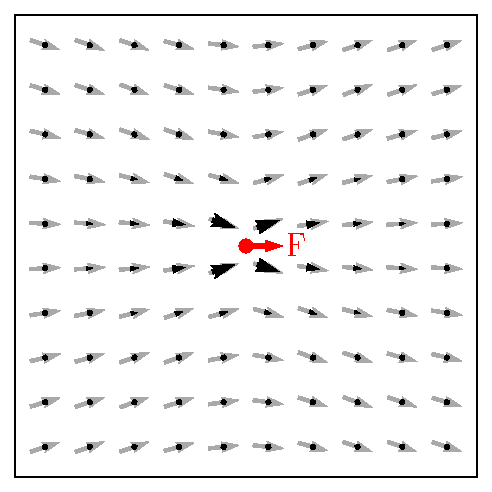
\includegraphics[width=0.49\columnwidth]{stokeslet1.pdf}
  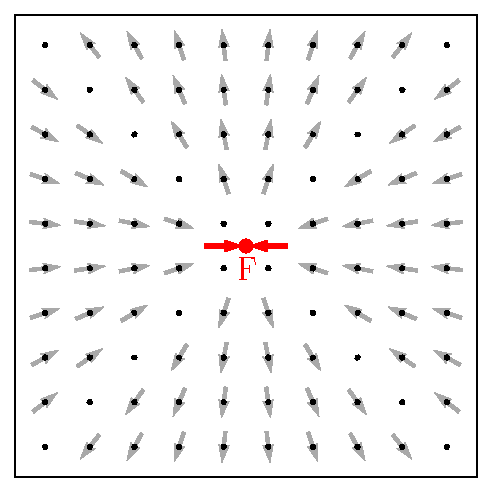
\includegraphics[width=0.49\columnwidth]{stresslet1.pdf}
  \caption{Flow fields due a Stokeslet (left) and a stresslet (right) centered at the origin (red dot). The black arrows display the velocities, while their directions are also indicated by the gray arrows. The flow fields are both axi- and fore-aft symmetric. Note the difference in the velocity magnitude of the two flows.}
  \label{fig:lets}
\end{figure}

Finally, for a sphere of radius $a$, translating with velocity $\bm U$ and rotating with angular velocity $\bm \Omega$, its total drag, torque, and stresslet are given by the \emph{Fax\'{e}n's laws},
\begin{subequations} \label{eq:faxen}
 \begin{equation}
   {\bm F}^{d} = 6\pi\mu a\bigg( (1+\frac{a^2}{6}\nabla^2){\bm u^\infty - {\bm U}} \bigg) ,
 \end{equation}
 \begin{equation}
  {\bm T}^{d} = 8\pi\mu a^3 ({\bm \omega}^\infty - {\bm \Omega}),
 \end{equation}
 \begin{equation}
   {\bm S} = \frac{20}{3}\pi\mu a^3 \bigg( 1+\frac{a^2}{10}\nabla^2 \bigg) {\bm E}^\infty ,
 \end{equation}
\end{subequations}
where $\small {\bm E}^\infty=(\nabla {\bm u}^\infty + (\nabla {\bm u}^\infty)^T)/2$ is the rate-of-strain tensor.


\section{Droplet interactions in shear flows}

The preceding section presents the most basic solutions of the Stokes flow when there is only one particle in the fluid.
In practice, however, it is rarely the case particles or droplets exist in isolation.
Particles tend to abound; and they often interact with each other through various types of hydrodynamic or non-hydrodynamic mechanisms giving rise to a multitude of phenomena in natural or artificial conditions.
For example, soap bubbles are always in a cluster due to the interfacial capillary attraction, while the same underlying principle can be applied to manipulate droplet motions on a surface to aid liquid handling \citep{vapour-sensing}.
To offer at least partial insights on the hydrodynamics, we highlight recent theoretical development of droplet interactions in bulk microflows, starting from the simplest case where two particles are immersed in unbounded simple shear flows.

Among the early studies of suspension flows, \cite{batchelor_green_1972} solved completely the dynamics of two rigid spheres of arbitrary size ratio subject to a background fluid motion whose velocity at infinity is a linear function of position, \ie
${\bm u}^\infty \sim {\bm E}^\infty \cdot {\bm x} + {\bm \omega}^\infty \times {\bm x}$ as $\abs{{\bm x}} \to \infty$.
The solution entails the relative velocity of the two sphere centers and the force dipole strengths of the two spheres (related to the effective viscosity of the suspension, see Section \ref{sec:sus-rheo}), and is given in terms of several scalar parameters functions of their relative position and size ratio alone.
In the special case where the two spheres are of equal size, the relative velocity can be integrated numerically to yield a trajectory map similar to Figure \ref{fig:BG-traj}.
Here, two types of trajectories can be observed:
(i) an \emph{open} trajectory where the faster particle overtakes the slower one, but afterwards, they never meet again; and
(ii) a \emph{closed} trajectory where two particles stay bound and rotate around each other permanently regardless of how far they may separate temporarily.
It is interesting to note that, under such ideal conditions, the closed trajectory has an infinite volume; if the two particles are aligned in the flow direction at any time, they will stay bound.

\begin{figure}%[t]
  \centering
  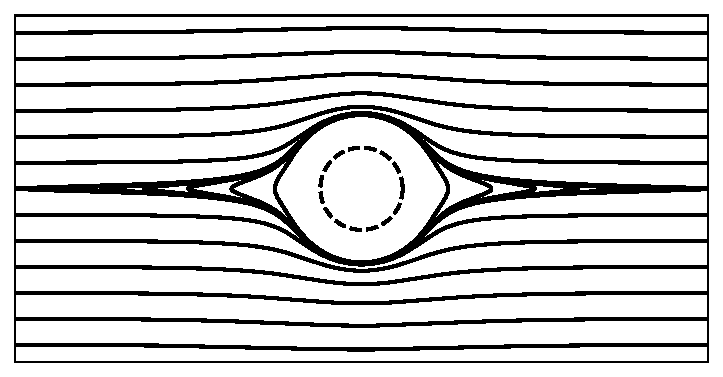
\includegraphics[width=0.8\columnwidth]{BG-traj4.pdf}
  \caption{Trajectory map of two equal spheres in unbounded simple shear flows. The dashed circle indicates the reference sphere, while the solid lines depict the relative trajectories of the second sphere in all planes of axisymmetry, which include the shear plane.}
  \label{fig:BG-traj}
\end{figure}

\cite{Zinchenko1983,Zinchenko1984} showed that essentially the same feature holds for liquid droplets.

With a distant wall, we show possibility of a stationary position.
Also dancing and swapping (\emph{Paper 4}). figure.
Here the wall can be considered as the third particle.
note the fact that the rate is very slow, since the relative velocity is small.

\begin{figure}%[t]
  \centering
  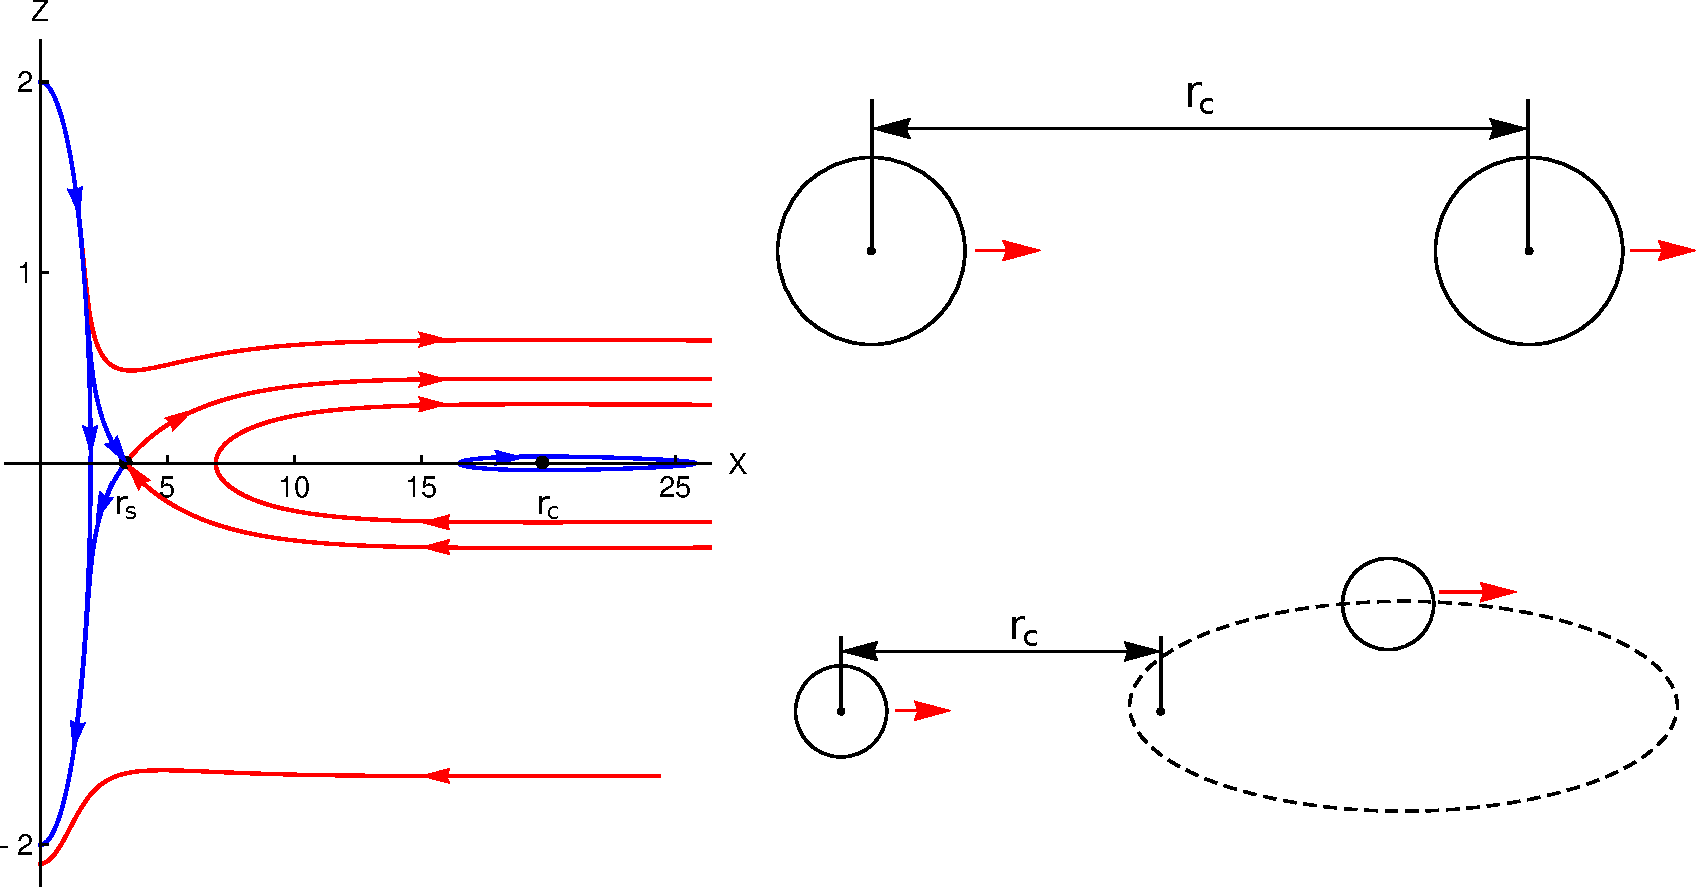
\includegraphics[width=0.9\columnwidth]{itzhak-boris.pdf}
  \caption{Trajectory map of two equal spheres in ...}
  \label{fig:itzhak-boris}
\end{figure}


With two walls, \cite{zurita-gotor_2007}
swapping.

We also show static pair under depletion force (\emph{Paper 2}).


\begin{figure}%[t]
  \centering
  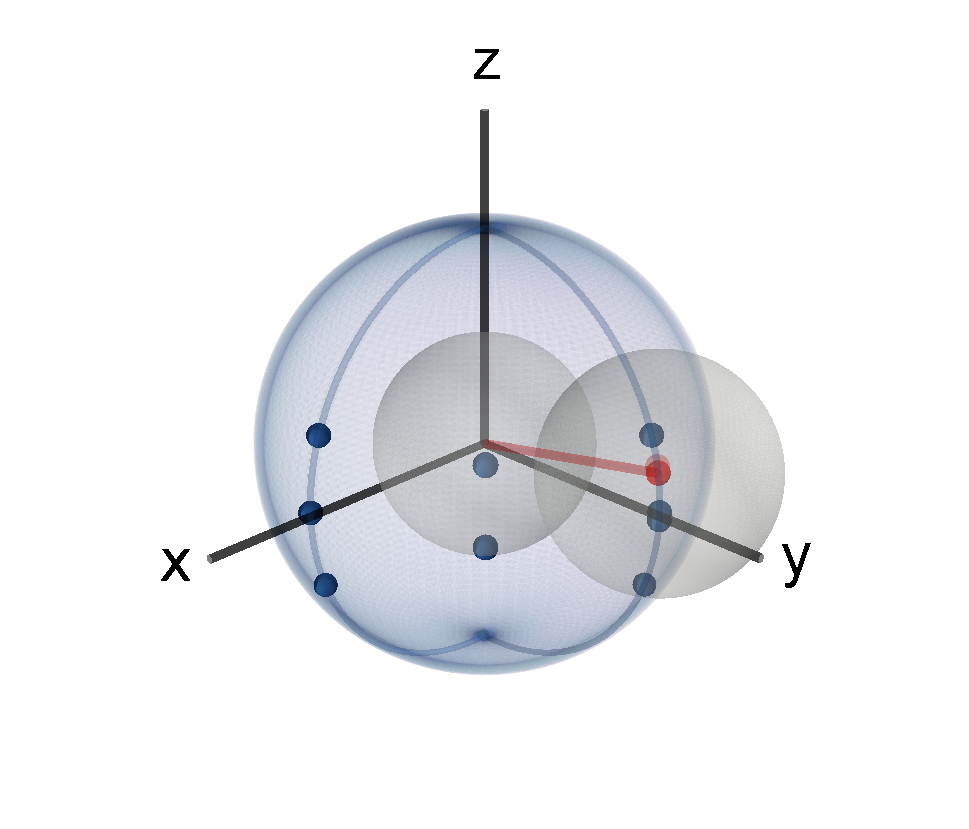
\includegraphics[width=0.3\columnwidth]{shell1.png}
  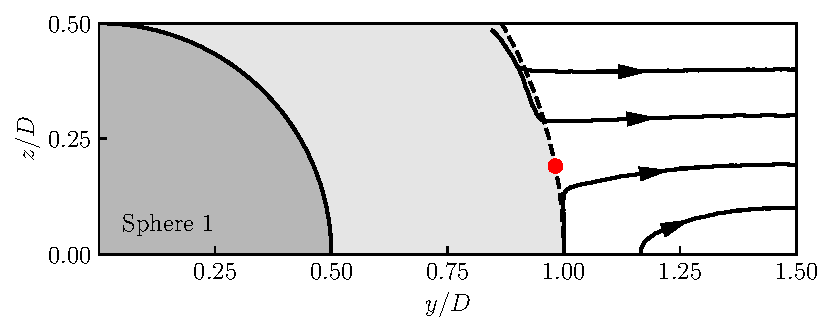
\includegraphics[width=0.6\columnwidth]{traj.pdf}
  \caption{Trajectory map of two droplets in ...}
  \label{fig:shear-align}
\end{figure}

even more confined:
dipolar theory \citep{Cui2004,Beatus2006,Janssen2012,Uspal2013,Desreumaux,zhu_gallaire_2016,q2d_Beatus,Diamant},
lubrication approximation.

range of interactions,


\section{Suspension rheology}
\label{sec:sus-rheo}

microstructure,
many-body problems (theoretical difficulties),
macroscopic properties, averages and bulk stresses (see Brady and Bossis).

The behaviour of systems involving the motion of small particles relative to a suspending fluid covers a wide range of phenomena of interest to both scientists and engineers. Dense suspensions, where the volume fraction of solid particles becomes comparable to or even higher than that of the fluid (see Figure \ref{fig:snap}), have particularly rich and sometimes unexpected rheologies, such as yielding, shear thinning, continuous shear thickening (CST), or discontinuous shear thickening (DST) \citep{mewis_wagner_book, Morton_Morris_2014, guazzelli_pouliquen_2018, Morris_annurev2020}. Apart from being theoretically intriguing, these complex behaviours often have major implications in practice. For instance, while it makes sense for the cement industry to manufacture suspensions that do not shear thicken, the same feature becomes an advantage for designing flexible body armor.



%===============================================================================
\chapter{Numerical Methods}
%===============================================================================



limitation of theoretical approaches,
necessity of numerical solutions.

Despite the practical importance, theoretical development of suspension rheology remains chanllenging and only a few analytical solutions have been found in the dilute regime, see \eg \cite{Einstein_1906, batchelor_green_1972b}. This is partially due to a lack of precise knowledge or control of various interactions at the particle level, partially due to the mathematical difficulties involved in many-body problems. On the other hand, solving a system of interacting particles is relatively straightforward in an algorithmic perspective. In fact, the last decades have seen tremendous advancement in both numerical simulations and computer hardware.

governing equations.

numerical solutions.


%-------------------------------------------------------------------------------

\section{Fluid-resolved methods}

level set methods,
(interface-correction level set/ghost fluid method),
volume-of-fluid methods,
phase-field methods,
immersed boundary methods.


\section{Particle-based methods}

The central equation to solve is
\begin{equation} 
 \begin{aligned} \label{eq:force-balance}
  {\bm m} \cdot \frac{d{\bm U}}{dt} = {\bm F}^H + {\bm F}^P, 
 \end{aligned}
\end{equation}
where ${\bm m}$ is a generalized mass/moment-of-inertia matrix of dimension $6N \times 6N$,
${\bm U}$ is the particle translational/rotational velocity vector of dimension $6N$,
and ${\bm F}$ represent the $6N$ force/torque vectors owing to hydrodynamics (denoted with superscript $\footnotesize H$) or other interactions (denoted with superscript $\footnotesize P$). Specifically, ${\bm F}^P$ may include contact, electrostatic, van der Waars, or magnetic forces, \etc. In principle, stochastic forces can also be included in the general formulation, though its numerical treatments demand special care such that fluctuation-dissipation theorem is satified. In the present thesis, Brownian motions are neglected.

For inertialess particles in Stokes flow, the task is to solve Eq.\ \eqref{eq:force-balance} subject to ${\bm m} \cdot (d{\bm U}/dt) \to 0$. Various techniques exist as summarized below.

\subsection{Stokesian dynamics}

The Stokesian dynamics \citep{Brady_Bossis1988} employs the fact that, when the particle Reynolds number is small and the bulk flow is linear, the hydrodynamic forces and stresses exerted on the particles by the fluid can be expressed as
\begin{equation} 
 \begin{aligned} \label{eq:sd-hydro}
  \begin{pmatrix}
   {\bm F}^H \\
   {\bm S}^H
  \end{pmatrix}
  = - \mathscr{R} \cdot
  \begin{pmatrix}
   {\bm U}-{\bm U}^\infty \\
   -{\bm E}^\infty
  \end{pmatrix},
 \end{aligned}
\end{equation}
where
\begin{equation} 
 \begin{aligned}
  \mathscr{R} =
  \begin{pmatrix}
   {\bm R}_{FU} & {\bm R}_{FE} \\
   {\bm R}_{SU} & {\bm R}_{SE}
  \end{pmatrix},
 \end{aligned}
\end{equation}
is termed the ``grand resistance'' matrix. 
If $\mathscr{R}$ is known, 
formulate the problem as

It is calculated as
\begin{equation} 
 \begin{aligned}
  \mathscr{R} = (\mathscr{M}^\infty)^{-1} +\mathscr{R}_{2B} - \mathscr{R}_{2B}^\infty.
 \end{aligned}
\end{equation}          
Es.\ \eqref{eq:sd-hydro} is then inverted and integrated in time to obtain the dynamics.


\subsection{Dissipative particle dynamics}

dissipative particle dynamics (DPD) \citep{Hoogerbrugge_1992, Groot_Warren_1997}


\subsection{Discrete element methods}


discrete element methods (DEM) \citep{Mari_Seto_2014JoR, Cheal_Ness_2018}, to name a few.
 the discrete-element lubrication/contact dynamics (DLCD) model.




%===============================================================================
\chapter{Summary}
%===============================================================================






%%===============================================================================
%\chapter{Test chapter, a very very very long title to test the table of contents}
%%===============================================================================
%
%This chapter is meant for testing the correct referencing of figures, equations
%and tables.
%
%% equations
%%
%\begin{equation}
%	1 + 1 = 2
%	\label{eq:test_eq1}
%\end{equation}
%
%\begin{align}
%	2 + 2 = 4
%	\label{eq:test_eq2}
%\end{align}
%
%\begin{equation}
%	3 + 3 = 6
%	\label{eq:test_eq3_intro}
%\end{equation}
%
%% tables
%%
%\begin{table}
%	\centering
%	\begin{tabular}{c}
%		1
%	\end{tabular}
%	\caption{Test table 1}
%	\label{tab:test_tab1}
%\end{table}
%
%\begin{table}
%	\centering
%	\begin{tabular}{c}
%		2
%	\end{tabular}
%	\caption{Test table 2}
%	\label{tab:test_tab2}
%\end{table}
%
%\begin{table}
%	\centering
%	\begin{tabular}{c}
%		3
%	\end{tabular}
%	\caption{Test table 3}
%	\label{tab:test_tab3_intro}
%\end{table}
%
%% figures
%%
%\begin{figure}[h!]
%	\centering
%	test figure 1
%	\caption{Test figure 1}
%	\label{fig:test_fig1}
%\end{figure}
%
%\begin{figure}[h!]
%	\centering
%	test figure 2
%	\caption{Test figure 2}
%	\label{fig:test_fig2}
%\end{figure}
%
%\begin{figure}[h!]
%	\centering
%	test figure 3
%	\caption{Test figure 3}
%	\label{fig:test_fig3_intro}
%\end{figure}
%
%% test references
%%
%\hrule
%\begin{itemize}
%	\item reference to equation 1: \eqref{eq:test_eq1}
%	\item reference to equation 2: \eqref{eq:test_eq2}
%	\item reference to equation 3: \eqref{eq:test_eq3_intro}
%\end{itemize}
%\hrule
%\begin{itemize}
%	\item reference to table 1: \eqref{tab:test_tab1}
%	\item reference to table 2: \eqref{tab:test_tab2}
%	\item reference to table 3: \eqref{tab:test_tab3_intro}
%\end{itemize}
%\hrule
%\begin{itemize}
%	\item reference to figure 1: \eqref{fig:test_fig1}
%	\item reference to figure 2: \eqref{fig:test_fig2}
%	\item reference to figure 3: \eqref{fig:test_fig3_intro}
%\end{itemize}
%\hrule

%===============================================================================
% Acknowledgments
%===============================================================================
%
\begin{acknowledgements}
%  Advisors,
%  funders,
%  collaborators,
%  mentors,
%  colleagues,
%  friends,
%  family.

  The first part of this thesis was written from December 2019 to January 2020, during the warmest winter since I arrived in Stockholm five years ago.
  Looking back, I have encountered, experienced and learned so much from uncountable people that is nearly impossible to name them one by one.
  I am grateful to \emph{everyone} and apologize in advance for any negligence.

  First and foremost, I thank Professor Luca Brandt for accepting me in and guiding me through the PhD program at KTH Mechanics.
  His strong leadership from the inception,
  enthusiastic responses and constructive criticisms at every discussion,
  generous support and increasing trust in me towards the end are indispensable for me to grow and develop academically.
  For these reasons, I owe my deepest gratitude to him.

  Second, I wish to extend my sincere thanks to my day-to-day advisors and mentors at KTH.
  I thank Outi Tammisolar for co-advising me since my first project, following my progress throughout the PhD
  and offering me invaluable career advice in the later years.
  I thank Jean-Christophe Loiseau for instilling in me the European culture, proper programming and mathematical rigour.
  I also thank Mehdi Niazi for always being available for technical discussions or code debugging and sharing his wisdom whenever I am lost.
  The patience, support and encouragement they offered me are instrumental in building my confidence and independence, which I will never take for granted.

  Third, I want to express my appreciation to all collaborators and senior colleagues that have shaped and contributed to my PhD work.
  These include, but are not limited to, international collaborators: Michael Dodd, Alexander Leshansky, Itzhak Fouxon and Naoki Takeishi;
  former and present colleagues at KTH: Walter Fornari, Pedro Costa, Francesco de Vita, Marco Rosti, B. M. Ningegowda and U\'{g}is L\={a}cis;
  office mates: Ricardo Vinuesa, Ekaterina Ezhova, Tímea Kékesi, Arash Alizad Banaei and Ashwin Vishnu;
  and professors that I enjoy talking to or playing innebandy with:
  Shervin Bagheri, Christophe Duwig, Hanno Essén, Nicholas Apazidis, Lanie Gutierrez-Farewik and Fredrik Lundell.
  Many others have also helped, corrected or inspired me in various research projects;
  my thanks are expressed in the separate acknowledgements after each paper in the next part of the thesis.
  
  In his famous essay, \emph{\small The World As I See It}, Einstein wrote,
  ``But from the point of view of daily life, without going deeper, we exist for our fellowmen --
  in the first place for those on whose smiles and welfare all our happiness depends,
  and next for all those unknown to us personally with whose destinies we are bound up by the tie of sympathy.''
  In the last several years, I have been lucky to derive plentiful happiness and sympathy from Artem, Erik, Guillaume, Nicolas, Frida, Natasha, Thea, Lee,
  as well as the rest of the Roslagstullsbacken corridor.
  Particularly, I am blessed to meet Dia, whose courage, ambition, curiosity and sensitivity have become a continuing source of my attachment,
  making me feel thorough and complete.
  
  Finally, none of the above would have been possible without the enduring love, hope, protection and education from my family at home.
  
  \chinese{爸,妈}
  
  \chinese{感谢你们对我从小到大的培养}

  \chinese{感谢你们对我的一切付出}

  \chinese{我的所有都属于你们}
  
  
\end{acknowledgements}



%===============================================================================
% References
%===============================================================================
%
\bibliographystyle{jfm}
\bibliography{thesis}
%
\IfFileExists{overview.bbl}{\graphicspath{{imgs/}}

%===============================================================================
\chapter{Introduction}
%===============================================================================



In \cite{Batchelor} we believe.


%-------------------------------------------------------------------------------

\section{Flow-assist droplet assembly}

material science,
photonic crystals,
microfluidics,
lab-on-a-chip.


\section{Liquid-infused surfaces}

drag reduction,
surface engineering,
superhydrophobicity,
lubricant-infused surfaces.


\section{Suspension flows}

particle suspensions,
complex fluids,
rheology,
shear thickening.

\thesisstructure Add here a brief description of the structure of the thesis.



%===============================================================================
\chapter{Microhydrodynamics}
%===============================================================================


In this chapter, we give a brief theoretical background of the topics studied.

mention the abuse of terms between droplets and particles.

The incompressible Navier-Stokes equation
\begin{subequations}
 \begin{equation}
   \nabla \cdot {\bm u} = 0,
  \label{eq:div-free}
 \end{equation}
 \begin{equation}
   \rho \bigg(\frac{\partial {\bm u}}{\partial t} + {\bm u} \cdot \nabla {\bm u} \bigg) = -\nabla p + \mu \nabla ^2  {\bm u} + {\bm f},
  \label{eq:NS}
 \end{equation}
\end{subequations}
governs the dynamics of Newtonian fluids (which is what we consider throughout the thesis).
where...

boundary conditions... between fluid and solid: continuity of the tangential velocity, \ie the no-slip condition (molecular slip ignored).
with an interface... surface tension... free surface... a boundary condition for the stress (see \cite{Batchelor} Sec.\ 3.3).


the Reynolds, Weber, and Froude numbers, defined as
\begin{equation}
  \begin{aligned}
    Re = \frac{\tilde{\rho} \tilde{U} \tilde{L}}{\tilde{\mu}},\quad \quad We = \frac{\tilde{\rho} \tilde{U}^2 \tilde{L}}{\tilde{\sigma}},\quad \quad Fr=\frac{\tilde{U}^2}{\tilde{g}\tilde{L}},      
  \label{eq:non-di-num}    
  \end{aligned}
\end{equation}
\noindent where $\tilde{U}$, $\tilde{L}$, $\tilde{\rho_1}$, $\tilde{\mu_1}$, and $\tilde{g}$ denote the reference dimensional velocity, length, density, dynamic viscosity, and gravitational acceleration. Note that $\rho_1=1$ and $\mu_1=1$ (i.e.\ we define fluid 1 as the reference fluid).
Perhaps also mention the Stouhal number.



%-------------------------------------------------------------------------------

\section{Stokes flow and its symmetries}

When small Reynolds number, Eq.\ \eqref{eq:NS} reduces to the Stokes equation,
\begin{equation}
   -\nabla p + \mu \nabla ^2  {\bm u} + {\bm f} = {\bm 0},
 \label{eq:Stokes}
\end{equation}
or, equivalently
\begin{equation}
   \nabla \cdot  {\bm \sigma} + {\bm f} = {\bm 0},
 \label{eq:Stokes1}
\end{equation}
where...

Stokes flow has the following symmetries and properties.
\begin{enumerate}
 \item \emph{Linearity}, which renders the applicability of superposition principle. For example, if $({\bm u}_1,p_1)$ is a solution to ${\bm f}={\bm f}_1$ and $({\bm u}_2,p_2)$ is a solution to ${\bm f}={\bm f}_2$, then $(\alpha{\bm u}_1+\beta {\bm u}_2,\alpha p_1 + \beta p_2)$ is a solution to ${\bm f}=\alpha{\bm f}_1 + \beta {\bm f}_2$.
 \item \emph{Reversibility}, which follows from the linearity and entails that, if the forcing changes from ${\bm f}$ to $-{\bm f}$, then the flow should reverse, \ie $({\bm u},p) \to (-{\bm u},-p)$. Note that, the simple reversibility symmetry can be very useful in deducing qualitative results without doing any calulation, see \eg the much celebrated note of \cite{Purcell1977}
 \item \emph{Stress equilibrium}, which states that any force exerted within the fluid is transmitted instantaneously to the boundary or, if there is no boundary, to infinity \citep{graham_2018}.
 \item \emph{Lorentz reciprocal relation}, which relates two solutions, $({\bm u}', {\bm \sigma}')$ and $({\bm u}'', {\bm \sigma}'')$ (they may differ by boundary conditions), of the Stokes equation by,
 \begin{equation}
  \small
  \begin{aligned}
   \int_V \bigg({\bm u}' \cdot (\nabla  \cdot {\bm \sigma}'') - {\bm u}'' \cdot (\nabla  \cdot {\bm \sigma}')\bigg) dV  & =\\
   \int_S \bigg({\bm u}' \cdot ({\bm n} \cdot {\bm \sigma}'') - {\bm u}'' \cdot ({\bm n} \cdot {\bm \sigma}')\bigg) dS, & 
  \end{aligned} \label{eq:lorentz-recip}
 \end{equation}
 where $V$ is some enclosed volume with surface $S$.
 \item \emph{Minimum dissipation principle}, which is a variational principle that asserts that the flow that minimizes energy dissipation rate subject to incompressibility and certain boundary conditions is the Stokes flow in that geometry.
\end{enumerate}


\section{Single particle in Stokes flow}

Green's function (Stoekslet),
stresslet (symmetric and traceless),
scaling laws (decay),
Fax\'{e}n's law,
confinement,
multipole expansion,
boundary integral methods.


\section{Particle interactions}

Batchelor and Green (1972),
swapping,
dancing,
range of interactions,
dipolar theory,
lubrication approximation.


\section{Rheology}

microstructure,
many-body problems (theoretical difficulties),
macroscopic properties, averages and bulk stresses (see Brady and Bossis).

The behaviour of systems involving the motion of small particles relative to a suspending fluid covers a wide range of phenomena of interest to both scientists and engineers. Dense suspensions, where the volume fraction of solid particles becomes comparable to or even higher than that of the fluid (see Figure \ref{fig:snap}), have particularly rich and sometimes unexpected rheologies, such as yielding, shear thinning, continuous shear thickening (CST), or discontinuous shear thickening (DST) \citep{mewis_wagner_book, Morton_Morris_2014, guazzelli_pouliquen_2018, Morris_annurev2020}. Apart from being theoretically intriguing, these complex behaviours often have major implications in practice. For instance, while it makes sense for the cement industry to manufacture suspensions that do not shear thicken, the same feature becomes an advantage for designing flexible body armor.



%===============================================================================
\chapter{Numerical Methods}
%===============================================================================



limitation of theoretical approaches,
necessity of numerical solutions.

Despite the practical importance, theoretical development of suspension rheology remains chanllenging and only a few analytical solutions have been found in the dilute regime, see \eg \cite{Einstein_1906, batchelor_green_1972b}. This is partially due to a lack of precise knowledge or control of various interactions at the particle level, partially due to the mathematical difficulties involved in many-body problems. On the other hand, solving a system of interacting particles is relatively straightforward in an algorithmic perspective. In fact, the last decades have seen tremendous advancement in both numerical simulations and computer hardware.

governing equations.

numerical solutions.


%-------------------------------------------------------------------------------

\section{Fluid-resolved methods}

level set methods,
(interface-correction level set/ghost fluid method),
volume-of-fluid methods,
phase-field methods,
immersed boundary methods.


\section{Particle-based methods}

The central equation to solve is
\begin{equation} 
 \begin{aligned} \label{eq:force-balance}
  {\bm m} \cdot \frac{d{\bm U}}{dt} = {\bm F}^H + {\bm F}^P, 
 \end{aligned}
\end{equation}
where ${\bm m}$ is a generalized mass/moment-of-inertia matrix of dimension $6N \times 6N$,
${\bm U}$ is the particle translational/rotational velocity vector of dimension $6N$,
and ${\bm F}$ represent the $6N$ force/torque vectors owing to hydrodynamics (denoted with superscript $\footnotesize H$) or other interactions (denoted with superscript $\footnotesize P$). Specifically, ${\bm F}^P$ may include contact, electrostatic, van der Waars, or magnetic forces, \etc. In principle, stochastic forces can also be included in the general formulation, though its numerical treatments demand special care such that fluctuation-dissipation theorem is satified. In the present thesis, Brownian motions are neglected.

For inertialess particles in Stokes flow, the task is to solve Eq.\ \eqref{eq:force-balance} subject to ${\bm m} \cdot (d{\bm U}/dt) \to 0$. Various techniques exist as summarized below.

\subsection{Stokesian dynamics}

The Stokesian dynamics \citep{Brady_Bossis1988} employs the fact that, when the particle Reynolds number is small and the bulk flow is linear, the hydrodynamic forces and stresses exerted on the particles by the fluid can be expressed as
\begin{equation} 
 \begin{aligned} \label{eq:sd-hydro}
  \begin{pmatrix}
   {\bm F}^H \\
   {\bm S}^H
  \end{pmatrix}
  = - \mathscr{R} \cdot
  \begin{pmatrix}
   {\bm U}-{\bm U}^\infty \\
   -{\bm E}^\infty
  \end{pmatrix},
 \end{aligned}
\end{equation}
where
\begin{equation} 
 \begin{aligned}
  \mathscr{R} =
  \begin{pmatrix}
   {\bm R}_{FU} & {\bm R}_{FE} \\
   {\bm R}_{SU} & {\bm R}_{SE}
  \end{pmatrix},
 \end{aligned}
\end{equation}
is termed the ``grand resistance'' matrix. 
If $\mathscr{R}$ is known, 
formulate the problem as

It is calculated as
\begin{equation} 
 \begin{aligned}
  \mathscr{R} = (\mathscr{M}^\infty)^{-1} +\mathscr{R}_{2B} - \mathscr{R}_{2B}^\infty.
 \end{aligned}
\end{equation}          
Es.\ \eqref{eq:sd-hydro} is then inverted and integrated in time to obtain the dynamics.


\subsection{Dissipative particle dynamics}

dissipative particle dynamics (DPD) \citep{Hoogerbrugge_1992, Groot_Warren_1997}


\subsection{Discrete element methods}


discrete element methods (DEM) \citep{Mari_Seto_2014JoR, Cheal_Ness_2018}, to name a few.
 the discrete-element lubrication/contact dynamics (DLCD) model.




%===============================================================================
\chapter{Summary}
%===============================================================================






%%===============================================================================
%\chapter{Test chapter, a very very very long title to test the table of contents}
%%===============================================================================
%
%This chapter is meant for testing the correct referencing of figures, equations
%and tables.
%
%% equations
%%
%\begin{equation}
%	1 + 1 = 2
%	\label{eq:test_eq1}
%\end{equation}
%
%\begin{align}
%	2 + 2 = 4
%	\label{eq:test_eq2}
%\end{align}
%
%\begin{equation}
%	3 + 3 = 6
%	\label{eq:test_eq3_intro}
%\end{equation}
%
%% tables
%%
%\begin{table}
%	\centering
%	\begin{tabular}{c}
%		1
%	\end{tabular}
%	\caption{Test table 1}
%	\label{tab:test_tab1}
%\end{table}
%
%\begin{table}
%	\centering
%	\begin{tabular}{c}
%		2
%	\end{tabular}
%	\caption{Test table 2}
%	\label{tab:test_tab2}
%\end{table}
%
%\begin{table}
%	\centering
%	\begin{tabular}{c}
%		3
%	\end{tabular}
%	\caption{Test table 3}
%	\label{tab:test_tab3_intro}
%\end{table}
%
%% figures
%%
%\begin{figure}[h!]
%	\centering
%	test figure 1
%	\caption{Test figure 1}
%	\label{fig:test_fig1}
%\end{figure}
%
%\begin{figure}[h!]
%	\centering
%	test figure 2
%	\caption{Test figure 2}
%	\label{fig:test_fig2}
%\end{figure}
%
%\begin{figure}[h!]
%	\centering
%	test figure 3
%	\caption{Test figure 3}
%	\label{fig:test_fig3_intro}
%\end{figure}
%
%% test references
%%
%\hrule
%\begin{itemize}
%	\item reference to equation 1: \eqref{eq:test_eq1}
%	\item reference to equation 2: \eqref{eq:test_eq2}
%	\item reference to equation 3: \eqref{eq:test_eq3_intro}
%\end{itemize}
%\hrule
%\begin{itemize}
%	\item reference to table 1: \eqref{tab:test_tab1}
%	\item reference to table 2: \eqref{tab:test_tab2}
%	\item reference to table 3: \eqref{tab:test_tab3_intro}
%\end{itemize}
%\hrule
%\begin{itemize}
%	\item reference to figure 1: \eqref{fig:test_fig1}
%	\item reference to figure 2: \eqref{fig:test_fig2}
%	\item reference to figure 3: \eqref{fig:test_fig3_intro}
%\end{itemize}
%\hrule

%===============================================================================
% Acknowledgments
%===============================================================================
%
\begin{acknowledgements}
%  Advisors,
%  funders,
%  collaborators,
%  mentors,
%  colleagues,
%  friends,
%  family.

  The first part of this thesis was written from December 2019 to January 2020, during the warmest winter since I arrived in Stockholm five years ago.
  Looking back, I have encountered, experienced and learned so much from uncountable people that is nearly impossible to name them one by one.
  I am grateful to \emph{everyone} and apologize in advance for any negligence.

  First and foremost, I thank Professor Luca Brandt for accepting me in and guiding me through the PhD program at KTH Mechanics.
  His strong leadership from the inception,
  enthusiastic responses and constructive criticisms at every discussion,
  generous support and increasing trust in me towards the end are indispensable for me to grow and develop academically.
  For these reasons, I owe my deepest gratitude to him.

  Second, I wish to extend my sincere thanks to my day-to-day advisors and mentors at KTH.
  I thank Outi Tammisolar for co-advising me since my first project, following my progress throughout the PhD
  and offering me invaluable career advice in the later years.
  I thank Jean-Christophe Loiseau for instilling in me the European culture, proper programming and mathematical rigour.
  I also thank Mehdi Niazi for always being available for technical discussions or code debugging and sharing his wisdom whenever I am lost.
  The patience, support and encouragement they offered me are instrumental in building my confidence and independence, which I will never take for granted.

  Third, I want to express my appreciation to all collaborators and senior colleagues that have shaped and contributed to my PhD work.
  These include, but are not limited to, international collaborators: Michael Dodd, Alexander Leshansky, Itzhak Fouxon and Naoki Takeishi;
  former and present colleagues at KTH: Walter Fornari, Pedro Costa, Francesco de Vita, Marco Rosti, B. M. Ningegowda and U\'{g}is L\={a}cis;
  office mates: Ricardo Vinuesa, Ekaterina Ezhova, Tímea Kékesi, Arash Alizad Banaei and Ashwin Vishnu;
  and professors that I enjoy talking to or playing innebandy with:
  Shervin Bagheri, Christophe Duwig, Hanno Essén, Nicholas Apazidis, Lanie Gutierrez-Farewik and Fredrik Lundell.
  Many others have also helped, corrected or inspired me in various research projects;
  my thanks are expressed in the separate acknowledgements after each paper in the next part of the thesis.
  
  In his famous essay, \emph{\small The World As I See It}, Einstein wrote,
  ``But from the point of view of daily life, without going deeper, we exist for our fellowmen --
  in the first place for those on whose smiles and welfare all our happiness depends,
  and next for all those unknown to us personally with whose destinies we are bound up by the tie of sympathy.''
  In the last several years, I have been lucky to derive plentiful happiness and sympathy from Artem, Erik, Guillaume, Nicolas, Frida, Natasha, Thea, Lee,
  as well as the rest of the Roslagstullsbacken corridor.
  Particularly, I am blessed to meet Dia, whose courage, ambition, curiosity and sensitivity have become a continuing source of my attachment,
  making me feel thorough and complete.
  
  Finally, none of the above would have been possible without the enduring love, hope, protection and education from my family at home.
  
  \chinese{爸,妈}
  
  \chinese{感谢你们对我从小到大的培养}

  \chinese{感谢你们对我的一切付出}

  \chinese{我的所有都属于你们}
  
  
\end{acknowledgements}



%===============================================================================
% References
%===============================================================================
%
\bibliographystyle{jfm}
\bibliography{thesis}
%
\IfFileExists{overview.bbl}{\graphicspath{{imgs/}}

%===============================================================================
\chapter{Introduction}
%===============================================================================



In \cite{Batchelor} we believe.


%-------------------------------------------------------------------------------

\section{Flow-assist droplet assembly}

material science,
photonic crystals,
microfluidics,
lab-on-a-chip.


\section{Liquid-infused surfaces}

drag reduction,
surface engineering,
superhydrophobicity,
lubricant-infused surfaces.


\section{Suspension flows}

particle suspensions,
complex fluids,
rheology,
shear thickening.

\thesisstructure Add here a brief description of the structure of the thesis.



%===============================================================================
\chapter{Microhydrodynamics}
%===============================================================================


In this chapter, we give a brief theoretical background of the topics studied.

mention the abuse of terms between droplets and particles.

The incompressible Navier-Stokes equation
\begin{subequations}
 \begin{equation}
   \nabla \cdot {\bm u} = 0,
  \label{eq:div-free}
 \end{equation}
 \begin{equation}
   \rho \bigg(\frac{\partial {\bm u}}{\partial t} + {\bm u} \cdot \nabla {\bm u} \bigg) = -\nabla p + \mu \nabla ^2  {\bm u} + {\bm f},
  \label{eq:NS}
 \end{equation}
\end{subequations}
governs the dynamics of Newtonian fluids (which is what we consider throughout the thesis).
where...

boundary conditions... between fluid and solid: continuity of the tangential velocity, \ie the no-slip condition (molecular slip ignored).
with an interface... surface tension... free surface... a boundary condition for the stress (see \cite{Batchelor} Sec.\ 3.3).


the Reynolds, Weber, and Froude numbers, defined as
\begin{equation}
  \begin{aligned}
    Re = \frac{\tilde{\rho} \tilde{U} \tilde{L}}{\tilde{\mu}},\quad \quad We = \frac{\tilde{\rho} \tilde{U}^2 \tilde{L}}{\tilde{\sigma}},\quad \quad Fr=\frac{\tilde{U}^2}{\tilde{g}\tilde{L}},      
  \label{eq:non-di-num}    
  \end{aligned}
\end{equation}
\noindent where $\tilde{U}$, $\tilde{L}$, $\tilde{\rho_1}$, $\tilde{\mu_1}$, and $\tilde{g}$ denote the reference dimensional velocity, length, density, dynamic viscosity, and gravitational acceleration. Note that $\rho_1=1$ and $\mu_1=1$ (i.e.\ we define fluid 1 as the reference fluid).
Perhaps also mention the Stouhal number.



%-------------------------------------------------------------------------------

\section{Stokes flow and its symmetries}

When small Reynolds number, Eq.\ \eqref{eq:NS} reduces to the Stokes equation,
\begin{equation}
   -\nabla p + \mu \nabla ^2  {\bm u} + {\bm f} = {\bm 0},
 \label{eq:Stokes}
\end{equation}
or, equivalently
\begin{equation}
   \nabla \cdot  {\bm \sigma} + {\bm f} = {\bm 0},
 \label{eq:Stokes1}
\end{equation}
where...

Stokes flow has the following symmetries and properties.
\begin{enumerate}
 \item \emph{Linearity}, which renders the applicability of superposition principle. For example, if $({\bm u}_1,p_1)$ is a solution to ${\bm f}={\bm f}_1$ and $({\bm u}_2,p_2)$ is a solution to ${\bm f}={\bm f}_2$, then $(\alpha{\bm u}_1+\beta {\bm u}_2,\alpha p_1 + \beta p_2)$ is a solution to ${\bm f}=\alpha{\bm f}_1 + \beta {\bm f}_2$.
 \item \emph{Reversibility}, which follows from the linearity and entails that, if the forcing changes from ${\bm f}$ to $-{\bm f}$, then the flow should reverse, \ie $({\bm u},p) \to (-{\bm u},-p)$. Note that, the simple reversibility symmetry can be very useful in deducing qualitative results without doing any calulation, see \eg the much celebrated note of \cite{Purcell1977}
 \item \emph{Stress equilibrium}, which states that any force exerted within the fluid is transmitted instantaneously to the boundary or, if there is no boundary, to infinity \citep{graham_2018}.
 \item \emph{Lorentz reciprocal relation}, which relates two solutions, $({\bm u}', {\bm \sigma}')$ and $({\bm u}'', {\bm \sigma}'')$ (they may differ by boundary conditions), of the Stokes equation by,
 \begin{equation}
  \small
  \begin{aligned}
   \int_V \bigg({\bm u}' \cdot (\nabla  \cdot {\bm \sigma}'') - {\bm u}'' \cdot (\nabla  \cdot {\bm \sigma}')\bigg) dV  & =\\
   \int_S \bigg({\bm u}' \cdot ({\bm n} \cdot {\bm \sigma}'') - {\bm u}'' \cdot ({\bm n} \cdot {\bm \sigma}')\bigg) dS, & 
  \end{aligned} \label{eq:lorentz-recip}
 \end{equation}
 where $V$ is some enclosed volume with surface $S$.
 \item \emph{Minimum dissipation principle}, which is a variational principle that asserts that the flow that minimizes energy dissipation rate subject to incompressibility and certain boundary conditions is the Stokes flow in that geometry.
\end{enumerate}


\section{Single particle in Stokes flow}

Green's function (Stoekslet),
stresslet (symmetric and traceless),
scaling laws (decay),
Fax\'{e}n's law,
confinement,
multipole expansion,
boundary integral methods.


\section{Particle interactions}

Batchelor and Green (1972),
swapping,
dancing,
range of interactions,
dipolar theory,
lubrication approximation.


\section{Rheology}

microstructure,
many-body problems (theoretical difficulties),
macroscopic properties, averages and bulk stresses (see Brady and Bossis).

The behaviour of systems involving the motion of small particles relative to a suspending fluid covers a wide range of phenomena of interest to both scientists and engineers. Dense suspensions, where the volume fraction of solid particles becomes comparable to or even higher than that of the fluid (see Figure \ref{fig:snap}), have particularly rich and sometimes unexpected rheologies, such as yielding, shear thinning, continuous shear thickening (CST), or discontinuous shear thickening (DST) \citep{mewis_wagner_book, Morton_Morris_2014, guazzelli_pouliquen_2018, Morris_annurev2020}. Apart from being theoretically intriguing, these complex behaviours often have major implications in practice. For instance, while it makes sense for the cement industry to manufacture suspensions that do not shear thicken, the same feature becomes an advantage for designing flexible body armor.



%===============================================================================
\chapter{Numerical Methods}
%===============================================================================



limitation of theoretical approaches,
necessity of numerical solutions.

Despite the practical importance, theoretical development of suspension rheology remains chanllenging and only a few analytical solutions have been found in the dilute regime, see \eg \cite{Einstein_1906, batchelor_green_1972b}. This is partially due to a lack of precise knowledge or control of various interactions at the particle level, partially due to the mathematical difficulties involved in many-body problems. On the other hand, solving a system of interacting particles is relatively straightforward in an algorithmic perspective. In fact, the last decades have seen tremendous advancement in both numerical simulations and computer hardware.

governing equations.

numerical solutions.


%-------------------------------------------------------------------------------

\section{Fluid-resolved methods}

level set methods,
(interface-correction level set/ghost fluid method),
volume-of-fluid methods,
phase-field methods,
immersed boundary methods.


\section{Particle-based methods}

The central equation to solve is
\begin{equation} 
 \begin{aligned} \label{eq:force-balance}
  {\bm m} \cdot \frac{d{\bm U}}{dt} = {\bm F}^H + {\bm F}^P, 
 \end{aligned}
\end{equation}
where ${\bm m}$ is a generalized mass/moment-of-inertia matrix of dimension $6N \times 6N$,
${\bm U}$ is the particle translational/rotational velocity vector of dimension $6N$,
and ${\bm F}$ represent the $6N$ force/torque vectors owing to hydrodynamics (denoted with superscript $\footnotesize H$) or other interactions (denoted with superscript $\footnotesize P$). Specifically, ${\bm F}^P$ may include contact, electrostatic, van der Waars, or magnetic forces, \etc. In principle, stochastic forces can also be included in the general formulation, though its numerical treatments demand special care such that fluctuation-dissipation theorem is satified. In the present thesis, Brownian motions are neglected.

For inertialess particles in Stokes flow, the task is to solve Eq.\ \eqref{eq:force-balance} subject to ${\bm m} \cdot (d{\bm U}/dt) \to 0$. Various techniques exist as summarized below.

\subsection{Stokesian dynamics}

The Stokesian dynamics \citep{Brady_Bossis1988} employs the fact that, when the particle Reynolds number is small and the bulk flow is linear, the hydrodynamic forces and stresses exerted on the particles by the fluid can be expressed as
\begin{equation} 
 \begin{aligned} \label{eq:sd-hydro}
  \begin{pmatrix}
   {\bm F}^H \\
   {\bm S}^H
  \end{pmatrix}
  = - \mathscr{R} \cdot
  \begin{pmatrix}
   {\bm U}-{\bm U}^\infty \\
   -{\bm E}^\infty
  \end{pmatrix},
 \end{aligned}
\end{equation}
where
\begin{equation} 
 \begin{aligned}
  \mathscr{R} =
  \begin{pmatrix}
   {\bm R}_{FU} & {\bm R}_{FE} \\
   {\bm R}_{SU} & {\bm R}_{SE}
  \end{pmatrix},
 \end{aligned}
\end{equation}
is termed the ``grand resistance'' matrix. 
If $\mathscr{R}$ is known, 
formulate the problem as

It is calculated as
\begin{equation} 
 \begin{aligned}
  \mathscr{R} = (\mathscr{M}^\infty)^{-1} +\mathscr{R}_{2B} - \mathscr{R}_{2B}^\infty.
 \end{aligned}
\end{equation}          
Es.\ \eqref{eq:sd-hydro} is then inverted and integrated in time to obtain the dynamics.


\subsection{Dissipative particle dynamics}

dissipative particle dynamics (DPD) \citep{Hoogerbrugge_1992, Groot_Warren_1997}


\subsection{Discrete element methods}


discrete element methods (DEM) \citep{Mari_Seto_2014JoR, Cheal_Ness_2018}, to name a few.
 the discrete-element lubrication/contact dynamics (DLCD) model.




%===============================================================================
\chapter{Summary}
%===============================================================================






%%===============================================================================
%\chapter{Test chapter, a very very very long title to test the table of contents}
%%===============================================================================
%
%This chapter is meant for testing the correct referencing of figures, equations
%and tables.
%
%% equations
%%
%\begin{equation}
%	1 + 1 = 2
%	\label{eq:test_eq1}
%\end{equation}
%
%\begin{align}
%	2 + 2 = 4
%	\label{eq:test_eq2}
%\end{align}
%
%\begin{equation}
%	3 + 3 = 6
%	\label{eq:test_eq3_intro}
%\end{equation}
%
%% tables
%%
%\begin{table}
%	\centering
%	\begin{tabular}{c}
%		1
%	\end{tabular}
%	\caption{Test table 1}
%	\label{tab:test_tab1}
%\end{table}
%
%\begin{table}
%	\centering
%	\begin{tabular}{c}
%		2
%	\end{tabular}
%	\caption{Test table 2}
%	\label{tab:test_tab2}
%\end{table}
%
%\begin{table}
%	\centering
%	\begin{tabular}{c}
%		3
%	\end{tabular}
%	\caption{Test table 3}
%	\label{tab:test_tab3_intro}
%\end{table}
%
%% figures
%%
%\begin{figure}[h!]
%	\centering
%	test figure 1
%	\caption{Test figure 1}
%	\label{fig:test_fig1}
%\end{figure}
%
%\begin{figure}[h!]
%	\centering
%	test figure 2
%	\caption{Test figure 2}
%	\label{fig:test_fig2}
%\end{figure}
%
%\begin{figure}[h!]
%	\centering
%	test figure 3
%	\caption{Test figure 3}
%	\label{fig:test_fig3_intro}
%\end{figure}
%
%% test references
%%
%\hrule
%\begin{itemize}
%	\item reference to equation 1: \eqref{eq:test_eq1}
%	\item reference to equation 2: \eqref{eq:test_eq2}
%	\item reference to equation 3: \eqref{eq:test_eq3_intro}
%\end{itemize}
%\hrule
%\begin{itemize}
%	\item reference to table 1: \eqref{tab:test_tab1}
%	\item reference to table 2: \eqref{tab:test_tab2}
%	\item reference to table 3: \eqref{tab:test_tab3_intro}
%\end{itemize}
%\hrule
%\begin{itemize}
%	\item reference to figure 1: \eqref{fig:test_fig1}
%	\item reference to figure 2: \eqref{fig:test_fig2}
%	\item reference to figure 3: \eqref{fig:test_fig3_intro}
%\end{itemize}
%\hrule

%===============================================================================
% Acknowledgments
%===============================================================================
%
\begin{acknowledgements}
%  Advisors,
%  funders,
%  collaborators,
%  mentors,
%  colleagues,
%  friends,
%  family.

  The first part of this thesis was written from December 2019 to January 2020, during the warmest winter since I arrived in Stockholm five years ago.
  Looking back, I have encountered, experienced and learned so much from uncountable people that is nearly impossible to name them one by one.
  I am grateful to \emph{everyone} and apologize in advance for any negligence.

  First and foremost, I thank Professor Luca Brandt for accepting me in and guiding me through the PhD program at KTH Mechanics.
  His strong leadership from the inception,
  enthusiastic responses and constructive criticisms at every discussion,
  generous support and increasing trust in me towards the end are indispensable for me to grow and develop academically.
  For these reasons, I owe my deepest gratitude to him.

  Second, I wish to extend my sincere thanks to my day-to-day advisors and mentors at KTH.
  I thank Outi Tammisolar for co-advising me since my first project, following my progress throughout the PhD
  and offering me invaluable career advice in the later years.
  I thank Jean-Christophe Loiseau for instilling in me the European culture, proper programming and mathematical rigour.
  I also thank Mehdi Niazi for always being available for technical discussions or code debugging and sharing his wisdom whenever I am lost.
  The patience, support and encouragement they offered me are instrumental in building my confidence and independence, which I will never take for granted.

  Third, I want to express my appreciation to all collaborators and senior colleagues that have shaped and contributed to my PhD work.
  These include, but are not limited to, international collaborators: Michael Dodd, Alexander Leshansky, Itzhak Fouxon and Naoki Takeishi;
  former and present colleagues at KTH: Walter Fornari, Pedro Costa, Francesco de Vita, Marco Rosti, B. M. Ningegowda and U\'{g}is L\={a}cis;
  office mates: Ricardo Vinuesa, Ekaterina Ezhova, Tímea Kékesi, Arash Alizad Banaei and Ashwin Vishnu;
  and professors that I enjoy talking to or playing innebandy with:
  Shervin Bagheri, Christophe Duwig, Hanno Essén, Nicholas Apazidis, Lanie Gutierrez-Farewik and Fredrik Lundell.
  Many others have also helped, corrected or inspired me in various research projects;
  my thanks are expressed in the separate acknowledgements after each paper in the next part of the thesis.
  
  In his famous essay, \emph{\small The World As I See It}, Einstein wrote,
  ``But from the point of view of daily life, without going deeper, we exist for our fellowmen --
  in the first place for those on whose smiles and welfare all our happiness depends,
  and next for all those unknown to us personally with whose destinies we are bound up by the tie of sympathy.''
  In the last several years, I have been lucky to derive plentiful happiness and sympathy from Artem, Erik, Guillaume, Nicolas, Frida, Natasha, Thea, Lee,
  as well as the rest of the Roslagstullsbacken corridor.
  Particularly, I am blessed to meet Dia, whose courage, ambition, curiosity and sensitivity have become a continuing source of my attachment,
  making me feel thorough and complete.
  
  Finally, none of the above would have been possible without the enduring love, hope, protection and education from my family at home.
  
  \chinese{爸,妈}
  
  \chinese{感谢你们对我从小到大的培养}

  \chinese{感谢你们对我的一切付出}

  \chinese{我的所有都属于你们}
  
  
\end{acknowledgements}



%===============================================================================
% References
%===============================================================================
%
\bibliographystyle{jfm}
\bibliography{thesis}
%
\IfFileExists{overview.bbl}{\graphicspath{{imgs/}}

%===============================================================================
\chapter{Introduction}
%===============================================================================



In \cite{Batchelor} we believe.


%-------------------------------------------------------------------------------

\section{Flow-assist droplet assembly}

material science,
photonic crystals,
microfluidics,
lab-on-a-chip.


\section{Liquid-infused surfaces}

drag reduction,
surface engineering,
superhydrophobicity,
lubricant-infused surfaces.


\section{Suspension flows}

particle suspensions,
complex fluids,
rheology,
shear thickening.

\thesisstructure Add here a brief description of the structure of the thesis.



%===============================================================================
\chapter{Microhydrodynamics}
%===============================================================================


In this chapter, we give a brief theoretical background of the topics studied.

mention the abuse of terms between droplets and particles.

The incompressible Navier-Stokes equation
\begin{subequations}
 \begin{equation}
   \nabla \cdot {\bm u} = 0,
  \label{eq:div-free}
 \end{equation}
 \begin{equation}
   \rho \bigg(\frac{\partial {\bm u}}{\partial t} + {\bm u} \cdot \nabla {\bm u} \bigg) = -\nabla p + \mu \nabla ^2  {\bm u} + {\bm f},
  \label{eq:NS}
 \end{equation}
\end{subequations}
governs the dynamics of Newtonian fluids (which is what we consider throughout the thesis).
where...

boundary conditions... between fluid and solid: continuity of the tangential velocity, \ie the no-slip condition (molecular slip ignored).
with an interface... surface tension... free surface... a boundary condition for the stress (see \cite{Batchelor} Sec.\ 3.3).


the Reynolds, Weber, and Froude numbers, defined as
\begin{equation}
  \begin{aligned}
    Re = \frac{\tilde{\rho} \tilde{U} \tilde{L}}{\tilde{\mu}},\quad \quad We = \frac{\tilde{\rho} \tilde{U}^2 \tilde{L}}{\tilde{\sigma}},\quad \quad Fr=\frac{\tilde{U}^2}{\tilde{g}\tilde{L}},      
  \label{eq:non-di-num}    
  \end{aligned}
\end{equation}
\noindent where $\tilde{U}$, $\tilde{L}$, $\tilde{\rho_1}$, $\tilde{\mu_1}$, and $\tilde{g}$ denote the reference dimensional velocity, length, density, dynamic viscosity, and gravitational acceleration. Note that $\rho_1=1$ and $\mu_1=1$ (i.e.\ we define fluid 1 as the reference fluid).
Perhaps also mention the Stouhal number.



%-------------------------------------------------------------------------------

\section{Stokes flow and its symmetries}

When small Reynolds number, Eq.\ \eqref{eq:NS} reduces to the Stokes equation,
\begin{equation}
   -\nabla p + \mu \nabla ^2  {\bm u} + {\bm f} = {\bm 0},
 \label{eq:Stokes}
\end{equation}
or, equivalently
\begin{equation}
   \nabla \cdot  {\bm \sigma} + {\bm f} = {\bm 0},
 \label{eq:Stokes1}
\end{equation}
where...

Stokes flow has the following symmetries and properties.
\begin{enumerate}
 \item \emph{Linearity}, which renders the applicability of superposition principle. For example, if $({\bm u}_1,p_1)$ is a solution to ${\bm f}={\bm f}_1$ and $({\bm u}_2,p_2)$ is a solution to ${\bm f}={\bm f}_2$, then $(\alpha{\bm u}_1+\beta {\bm u}_2,\alpha p_1 + \beta p_2)$ is a solution to ${\bm f}=\alpha{\bm f}_1 + \beta {\bm f}_2$.
 \item \emph{Reversibility}, which follows from the linearity and entails that, if the forcing changes from ${\bm f}$ to $-{\bm f}$, then the flow should reverse, \ie $({\bm u},p) \to (-{\bm u},-p)$. Note that, the simple reversibility symmetry can be very useful in deducing qualitative results without doing any calulation, see \eg the much celebrated note of \cite{Purcell1977}
 \item \emph{Stress equilibrium}, which states that any force exerted within the fluid is transmitted instantaneously to the boundary or, if there is no boundary, to infinity \citep{graham_2018}.
 \item \emph{Lorentz reciprocal relation}, which relates two solutions, $({\bm u}', {\bm \sigma}')$ and $({\bm u}'', {\bm \sigma}'')$ (they may differ by boundary conditions), of the Stokes equation by,
 \begin{equation}
  \small
  \begin{aligned}
   \int_V \bigg({\bm u}' \cdot (\nabla  \cdot {\bm \sigma}'') - {\bm u}'' \cdot (\nabla  \cdot {\bm \sigma}')\bigg) dV  & =\\
   \int_S \bigg({\bm u}' \cdot ({\bm n} \cdot {\bm \sigma}'') - {\bm u}'' \cdot ({\bm n} \cdot {\bm \sigma}')\bigg) dS, & 
  \end{aligned} \label{eq:lorentz-recip}
 \end{equation}
 where $V$ is some enclosed volume with surface $S$.
 \item \emph{Minimum dissipation principle}, which is a variational principle that asserts that the flow that minimizes energy dissipation rate subject to incompressibility and certain boundary conditions is the Stokes flow in that geometry.
\end{enumerate}


\section{Single particle in Stokes flow}

Green's function (Stoekslet),
stresslet (symmetric and traceless),
scaling laws (decay),
Fax\'{e}n's law,
confinement,
multipole expansion,
boundary integral methods.


\section{Particle interactions}

Batchelor and Green (1972),
swapping,
dancing,
range of interactions,
dipolar theory,
lubrication approximation.


\section{Rheology}

microstructure,
many-body problems (theoretical difficulties),
macroscopic properties, averages and bulk stresses (see Brady and Bossis).

The behaviour of systems involving the motion of small particles relative to a suspending fluid covers a wide range of phenomena of interest to both scientists and engineers. Dense suspensions, where the volume fraction of solid particles becomes comparable to or even higher than that of the fluid (see Figure \ref{fig:snap}), have particularly rich and sometimes unexpected rheologies, such as yielding, shear thinning, continuous shear thickening (CST), or discontinuous shear thickening (DST) \citep{mewis_wagner_book, Morton_Morris_2014, guazzelli_pouliquen_2018, Morris_annurev2020}. Apart from being theoretically intriguing, these complex behaviours often have major implications in practice. For instance, while it makes sense for the cement industry to manufacture suspensions that do not shear thicken, the same feature becomes an advantage for designing flexible body armor.



%===============================================================================
\chapter{Numerical Methods}
%===============================================================================



limitation of theoretical approaches,
necessity of numerical solutions.

Despite the practical importance, theoretical development of suspension rheology remains chanllenging and only a few analytical solutions have been found in the dilute regime, see \eg \cite{Einstein_1906, batchelor_green_1972b}. This is partially due to a lack of precise knowledge or control of various interactions at the particle level, partially due to the mathematical difficulties involved in many-body problems. On the other hand, solving a system of interacting particles is relatively straightforward in an algorithmic perspective. In fact, the last decades have seen tremendous advancement in both numerical simulations and computer hardware.

governing equations.

numerical solutions.


%-------------------------------------------------------------------------------

\section{Fluid-resolved methods}

level set methods,
(interface-correction level set/ghost fluid method),
volume-of-fluid methods,
phase-field methods,
immersed boundary methods.


\section{Particle-based methods}

The central equation to solve is
\begin{equation} 
 \begin{aligned} \label{eq:force-balance}
  {\bm m} \cdot \frac{d{\bm U}}{dt} = {\bm F}^H + {\bm F}^P, 
 \end{aligned}
\end{equation}
where ${\bm m}$ is a generalized mass/moment-of-inertia matrix of dimension $6N \times 6N$,
${\bm U}$ is the particle translational/rotational velocity vector of dimension $6N$,
and ${\bm F}$ represent the $6N$ force/torque vectors owing to hydrodynamics (denoted with superscript $\footnotesize H$) or other interactions (denoted with superscript $\footnotesize P$). Specifically, ${\bm F}^P$ may include contact, electrostatic, van der Waars, or magnetic forces, \etc. In principle, stochastic forces can also be included in the general formulation, though its numerical treatments demand special care such that fluctuation-dissipation theorem is satified. In the present thesis, Brownian motions are neglected.

For inertialess particles in Stokes flow, the task is to solve Eq.\ \eqref{eq:force-balance} subject to ${\bm m} \cdot (d{\bm U}/dt) \to 0$. Various techniques exist as summarized below.

\subsection{Stokesian dynamics}

The Stokesian dynamics \citep{Brady_Bossis1988} employs the fact that, when the particle Reynolds number is small and the bulk flow is linear, the hydrodynamic forces and stresses exerted on the particles by the fluid can be expressed as
\begin{equation} 
 \begin{aligned} \label{eq:sd-hydro}
  \begin{pmatrix}
   {\bm F}^H \\
   {\bm S}^H
  \end{pmatrix}
  = - \mathscr{R} \cdot
  \begin{pmatrix}
   {\bm U}-{\bm U}^\infty \\
   -{\bm E}^\infty
  \end{pmatrix},
 \end{aligned}
\end{equation}
where
\begin{equation} 
 \begin{aligned}
  \mathscr{R} =
  \begin{pmatrix}
   {\bm R}_{FU} & {\bm R}_{FE} \\
   {\bm R}_{SU} & {\bm R}_{SE}
  \end{pmatrix},
 \end{aligned}
\end{equation}
is termed the ``grand resistance'' matrix. 
If $\mathscr{R}$ is known, 
formulate the problem as

It is calculated as
\begin{equation} 
 \begin{aligned}
  \mathscr{R} = (\mathscr{M}^\infty)^{-1} +\mathscr{R}_{2B} - \mathscr{R}_{2B}^\infty.
 \end{aligned}
\end{equation}          
Es.\ \eqref{eq:sd-hydro} is then inverted and integrated in time to obtain the dynamics.


\subsection{Dissipative particle dynamics}

dissipative particle dynamics (DPD) \citep{Hoogerbrugge_1992, Groot_Warren_1997}


\subsection{Discrete element methods}


discrete element methods (DEM) \citep{Mari_Seto_2014JoR, Cheal_Ness_2018}, to name a few.
 the discrete-element lubrication/contact dynamics (DLCD) model.




%===============================================================================
\chapter{Summary}
%===============================================================================






%%===============================================================================
%\chapter{Test chapter, a very very very long title to test the table of contents}
%%===============================================================================
%
%This chapter is meant for testing the correct referencing of figures, equations
%and tables.
%
%% equations
%%
%\begin{equation}
%	1 + 1 = 2
%	\label{eq:test_eq1}
%\end{equation}
%
%\begin{align}
%	2 + 2 = 4
%	\label{eq:test_eq2}
%\end{align}
%
%\begin{equation}
%	3 + 3 = 6
%	\label{eq:test_eq3_intro}
%\end{equation}
%
%% tables
%%
%\begin{table}
%	\centering
%	\begin{tabular}{c}
%		1
%	\end{tabular}
%	\caption{Test table 1}
%	\label{tab:test_tab1}
%\end{table}
%
%\begin{table}
%	\centering
%	\begin{tabular}{c}
%		2
%	\end{tabular}
%	\caption{Test table 2}
%	\label{tab:test_tab2}
%\end{table}
%
%\begin{table}
%	\centering
%	\begin{tabular}{c}
%		3
%	\end{tabular}
%	\caption{Test table 3}
%	\label{tab:test_tab3_intro}
%\end{table}
%
%% figures
%%
%\begin{figure}[h!]
%	\centering
%	test figure 1
%	\caption{Test figure 1}
%	\label{fig:test_fig1}
%\end{figure}
%
%\begin{figure}[h!]
%	\centering
%	test figure 2
%	\caption{Test figure 2}
%	\label{fig:test_fig2}
%\end{figure}
%
%\begin{figure}[h!]
%	\centering
%	test figure 3
%	\caption{Test figure 3}
%	\label{fig:test_fig3_intro}
%\end{figure}
%
%% test references
%%
%\hrule
%\begin{itemize}
%	\item reference to equation 1: \eqref{eq:test_eq1}
%	\item reference to equation 2: \eqref{eq:test_eq2}
%	\item reference to equation 3: \eqref{eq:test_eq3_intro}
%\end{itemize}
%\hrule
%\begin{itemize}
%	\item reference to table 1: \eqref{tab:test_tab1}
%	\item reference to table 2: \eqref{tab:test_tab2}
%	\item reference to table 3: \eqref{tab:test_tab3_intro}
%\end{itemize}
%\hrule
%\begin{itemize}
%	\item reference to figure 1: \eqref{fig:test_fig1}
%	\item reference to figure 2: \eqref{fig:test_fig2}
%	\item reference to figure 3: \eqref{fig:test_fig3_intro}
%\end{itemize}
%\hrule

%===============================================================================
% Acknowledgments
%===============================================================================
%
\input{acknowledgements}


%===============================================================================
% References
%===============================================================================
%
\bibliographystyle{jfm}
\bibliography{thesis}
%
\IfFileExists{overview.bbl}{\input{overview.bbl}}{}
}{}
}{}
}{}
